\documentclass[a4paper,fleqn,usenatbib]{mnras}

%=========================================================================
\usepackage{amsmath} 
\usepackage{amssymb} 
\usepackage{graphicx}
\usepackage{grffile}
\usepackage[dvips]{epsfig}
\usepackage{epsfig}  
\usepackage{color}
\usepackage{caption}
\usepackage{hyperref}
\usepackage{bm}
%Non reposionated tables




%=========================================================================
%		INTERNAL MACROS
%=========================================================================
\def\be{\begin{equation}}
\def\ee{\end{equation}}
\def\ba{\begin{eqnarray}}
\def\ea{\end{eqnarray}}

% To highlight comments 
\definecolor{red}{rgb}{1,0.0,0.0}
\newcommand{\red}{\color{red}}
\definecolor{darkgreen}{rgb}{0.0,0.5,0.0}
\newcommand{\SRK}[1]{\textcolor{darkgreen}{\bf SRK: \textit{#1}}}
\newcommand{\SRKED}[1]{\textcolor{darkgreen}{\bf #1}}
\newcommand{\before}[1]{\textcolor{red}{ #1}}
\newcommand{\after}[1]{\textcolor{darkgreen}{ #1}}
\newcommand{\hs}{{\hspace{1mm}}}  
\newcommand{\tol}{Tololo 1214-277}
\newcommand{\HI}{{\text{H\MakeUppercase{\romannumeral 1}}} }
\newcommand{\HII}{{\text{H\MakeUppercase{\romannumeral 2}}} }
\newcommand{\lya}{\ifmmode{{\rm Ly}\alpha}\else Ly$\alpha$\ \fi}
\newcommand{\cm}{\ifmmode{{\rm cm}}\else cm\fi}
\newcommand{\ccm}{\,\mathrm{cm}^{-3}}
\newcommand{\ergps}{\,{\rm erg}\,{\rm s}\ifmmode{}^{-1}\else ${}^{-1}$\fi}
\newcommand{\Mpch}{\,{\rm Mpc}\,\ifmmode h^{-1}\else $h^{-1}$\fi}
\newcommand{\dd}{\mathrm{d}}
\newcommand{\vek}[1]{\bm{#1}}
\newcommand{\hb}{H$\beta$}
\newcommand{\ha}{H$\alpha$}
\newcommand{\oiii}{[OIII]}
\newcommand{\oii}{[OII]}
\newcommand{\nii}{[NII]}
\newcommand{\esca}{erg cm$^{-2}$ s$^{-1}$ \AA$^{-1}$}
\newcommand{\esc}{erg cm$^{-2}$ s$^{-1}$}
\newcommand{\es}{erg s$^{-1}$}
\newcommand{\esa}{erg s$^{-1}$}
\newcommand{\kms}{\ifmmode\mathrm{km\ s}^{-1}\else km s$^{-1}$\fi}
\newcommand{\hMsun}{{\ifmmode{h^{-1}{\rm{M_{\odot}}}}\else{$h^{-1}{\rm{M_{\odot}}}$}\fi}}
\newcommand{\Msun}{{\ifmmode{{\rm{M_{\odot}}}}\else{${\rm{M_{\odot}}}$}\fi}}

\newcommand{\jefr}[1]{\textcolor{darkgreen}{\bf JEFR: \textit{#1}}}

\begin{document}

%=========================================================================
%		FRONT MATTER
%=========================================================================
\title[Satellites in the MW and M31]{Joint Satellite Distributions in the Milky Way and Andromeda}
\author[J.E. Forero-Romero \& V. Arias]
{Jaime E. Forero-Romero $^{1}$ \thanks{je.forero@uniandes.edu.co},
Ver\'onica Arias$^1$\\
%%
$^1$ Departamento de F\'isica, Universidad de los Andes, Cra. 1
  No. 18A-10 Edificio Ip, CP 111711, Bogot\'a, Colombia \\
}

\maketitle

\begin{abstract}
We quantify the joint spatial distribution of satellites around the Milky way and Andromeda.
\end{abstract}

\begin{keywords}Galaxies: halos --- Galaxies: high-redshift --- Galaxies: statistics
--- Dark Matter --- Methods: numerical 
\end{keywords}

\section{Introduction}

\section{Observational Data}
\label{sec:obs}


\section{Local Group Satellites in the Illustris Simulation}
\label{sec:NumericalSetup}

We use publicly available data from the Illustris Project 
\citep{2014MNRAS.444.1518V}. 
This suite of cosmological simulations, performed using the quasi-Lagrangian
code AREPO \citep{2010MNRAS.401..791S}, followed the coupled evolution of dark 
matter and gas and includes parametrizations to account for the effects of
gas cooling, photoionization, star formation, stellar feedback, black
hole and super massive black hole feedback. 
The simulation volume is a cubic box of $75$ \Mpch\ on a side.
The cosmological parameters correspond to a $\Lambda$CDM cosmology
consistent with WMAP-9 measurements \citep{2013ApJS..208...19H}. 

We extract halo and galaxy information from the Illustris-1 simulation
which has the highest resolution in the current release of the
Illustris Project.
Illustris-1 has $1820^3$ dark matter particles and $1820^3$ initial gas
volumen elements. 
This corresponds to a dark matter particle mass of
$6.3\times 10^6$\Msun\ and a minimum mass for the baryonic volume
element of $8.0\times 10^7$\Msun. 
The corresponding spatial resolution is $1.4$ kpc for the dark matter
gravitational softening and $0.7$ kpc for the typical size of the
smallest gas cell size. 

The smallest satellites are barely resolved in stellar mass at magnitudes of
$M_V=9$, however its dark matter structure is sampled with at least
$100$ particles. 
We find that all considered halos have at least $XX$ subhalos above
a maximum circular velocity of $15$\kms.
For this reason we select the satellite galaxy samples from the
DM subhalo population and not from the galaxies with photometry.
We chose in two different ways the sub-halo samples. 
First, we rank the halos by decreasing order of its maximum circular
velocity and select the first $N_p$ halos in the list.
Second, we select all satellites above maximum circular velocity of
$20$\kms to randmbly subsample $N_p$ subhalos.


We build a sample of Local Group Analgues (LGA) by selecting first all
galaxies with  an stellar mass in the range $1\times10^{10}\Msun
<M_{\star}<1.5 \times 10^{11} \Msun$.
Then we consider the following criteria for all galaxies in that
sample.

\begin{itemize}
\item For each galaxy $A$ we find its closest galaxy $B$, if galaxy $A$ is also
the closest to halo $B$, the two are considered as a pair. 
\item With $d_{AB}$ the distance between the two galaxies and
  $M_{\star,min}$ the lowest stellar mass in the two galaxies, we
  discard pairs that have any other galaxy $C$ with stellar mas
  $M_{\star}>M_{\star, min}$ closer than $3\times d_{AB}$ from any of
  the pair's members.
\item The distance $d_{AB}>700$ kpc. 
\item The radial velocity between the two galaxies is $120\kms <V_{AB, radial}<0\kms$
\end{itemize}

We find $XX$ pairs with these conditions.




\section{Satellite Spatial Distribution and Alignment}
\label{sec:SpatialMeasurements}

We use the inertia tensor to characterize the satellites.
This tensor is defined as

\begin{equation}
{\bf{\bar{I}}} = \sum_{k \in V}[(\bf{r}_i - \bf{r}_0)^2\cdot \bf{1} -
  (\bf{r}_i-\bf{r}_0)\cdot (\bf{r}_i - \bf{r}_0)^{T}],
\end{equation}
%
where $k$ indexes the set of satellites of interest
$\bf{r}_k$ are the satellites' positions, $\bf{r}_{0}$ is the
positions pof the host DM halo, $\bf{1}$ is the unit matrix,  and
${\bf r}^T$ is the transposed vector $\bf{r}$. 
We finally compute the eigenvalues, $a>b>c$, and corresponding
eigenvectors, $\hat{I}_a$, $\hat{I}_b$, $\hat{I}_c$, of this tensor.
In the case of a sheet-like configuration the vector perpendicular to
the sheet would be signaled by, $\hat{I}_a$, the eigenvector of the
largest eigenvalue. 
We measure the width of the satellite distribution as the standard
deviation of all satellite distances to the plane defined by the
vector $\hat{I}_a$. 

% referencia posiciones satellites
% http://adsabs.harvard.edu/abs/2013MNRAS.435.1928P


\begin{table*}
  \centering
\begin{tabular}{lll}
\hline\hline
Symbol & Units & Description\\\hline
$\hat{r}_{AB}$& & Unit vector along the direction connecting two
dominant galaxies\\
$N_s$ & & Number of satellites\\
$a > b> c$ & & Inertia tensor eigenvalues. \\
$\hat{I}_a$, $\hat{I}_b$, $\hat{I}_c$ & & Inertia tensor eigenvectors. \\
$\sigma_s$ & kpc & Ellipsoid width\\
\hline\hline
\end{tabular}
  \caption{Overview of the parameters computed for each central galaxy
    and its satellite system.
  \label{tab:models}}
\end{table*}


\section{Results}
\label{sec:results}

\begin{figure*}
\centering
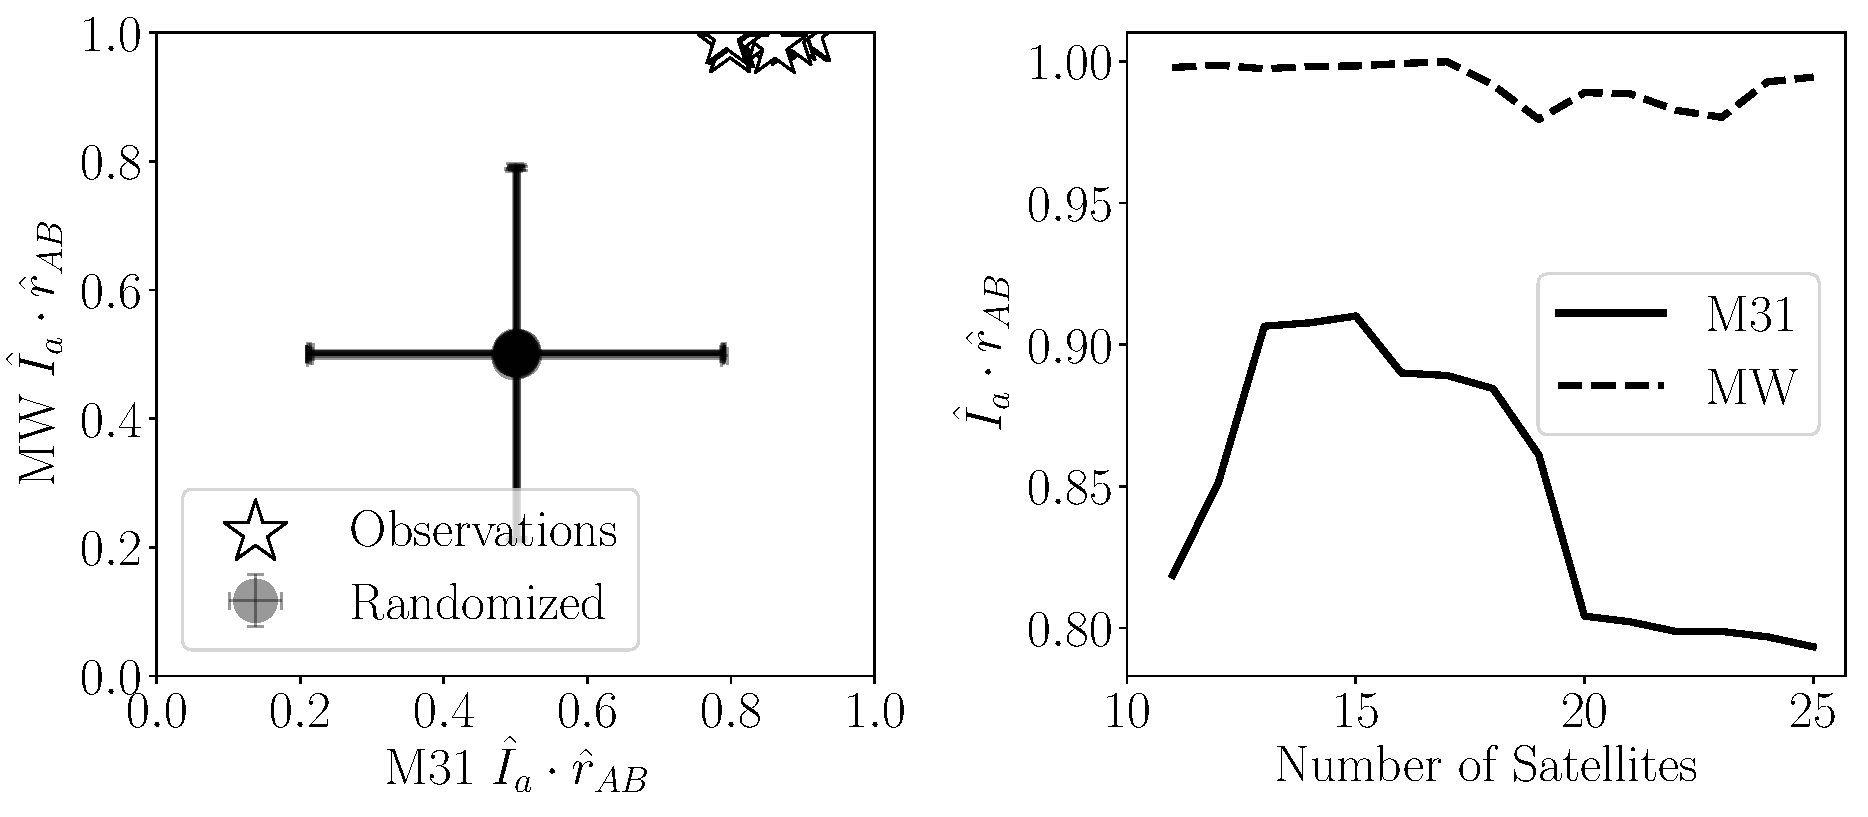
\includegraphics[width=0.7\textwidth]{mu_lg.pdf}
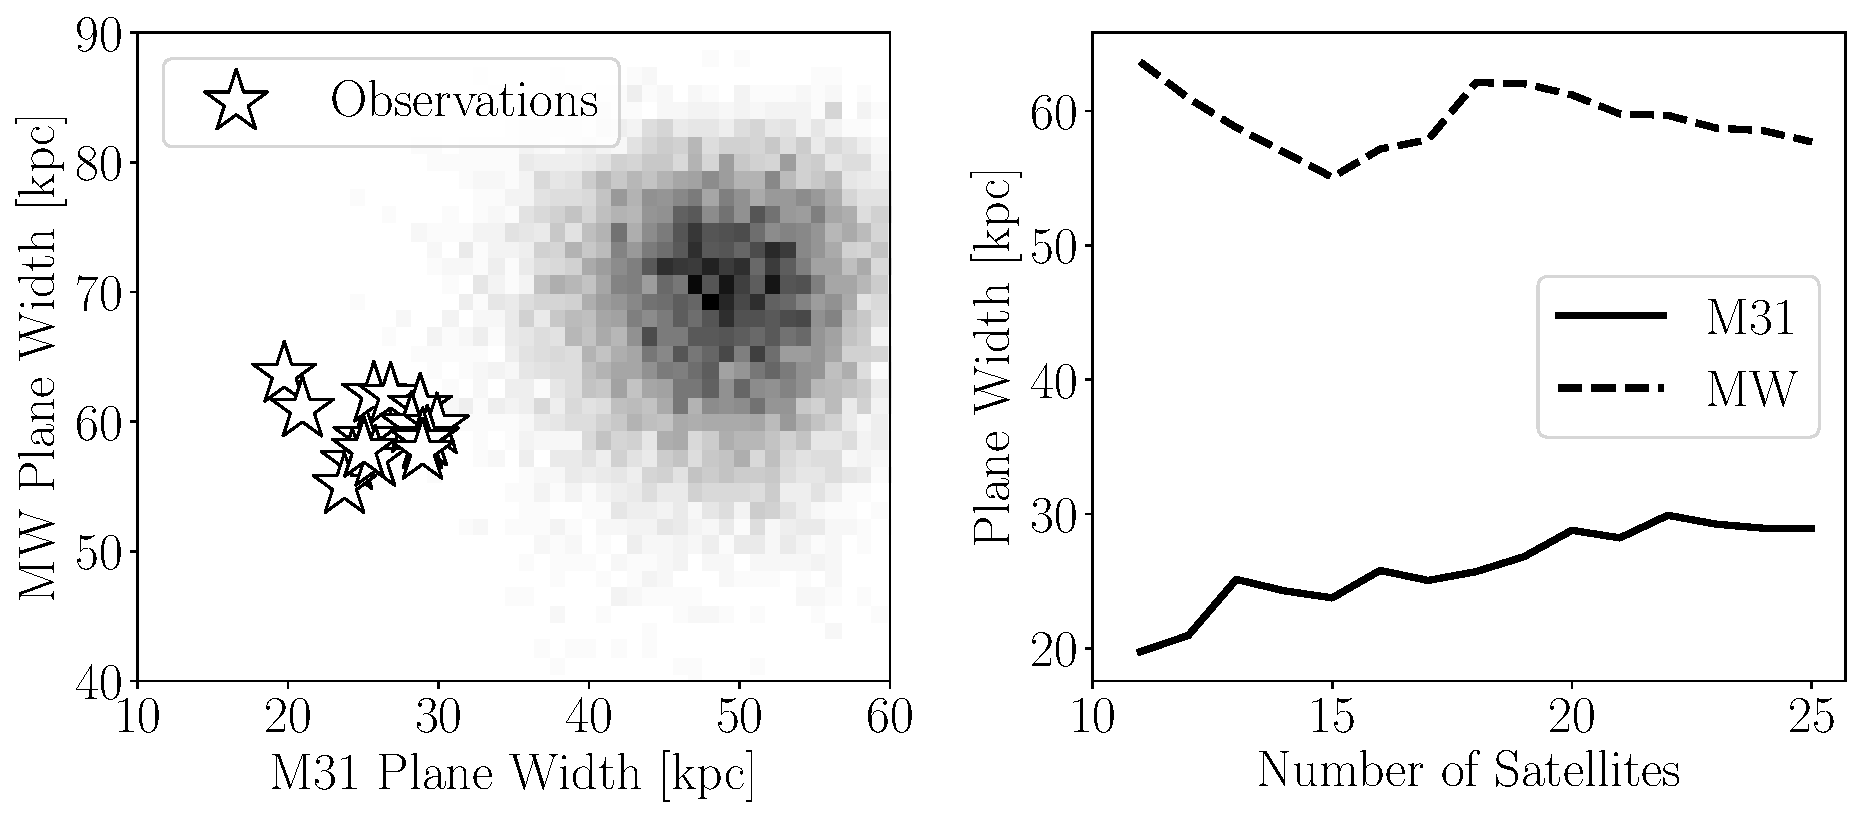
\includegraphics[width=0.7\textwidth]{planewidth_lg.pdf}
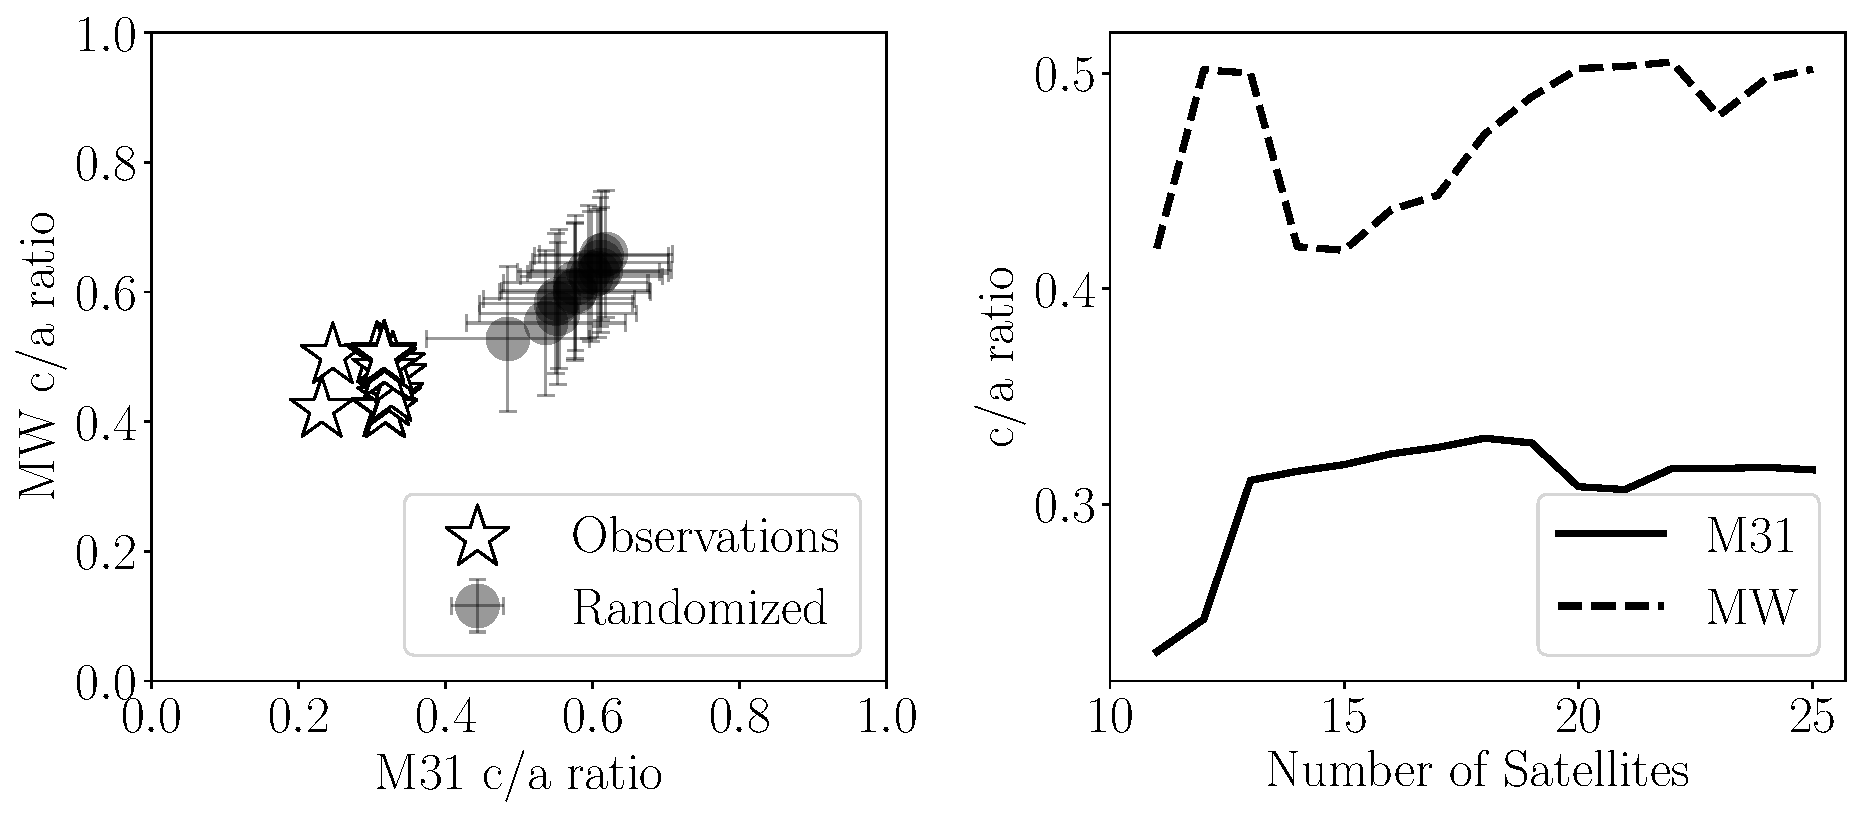
\includegraphics[width=0.7\textwidth]{ca_ratio_lg.pdf}
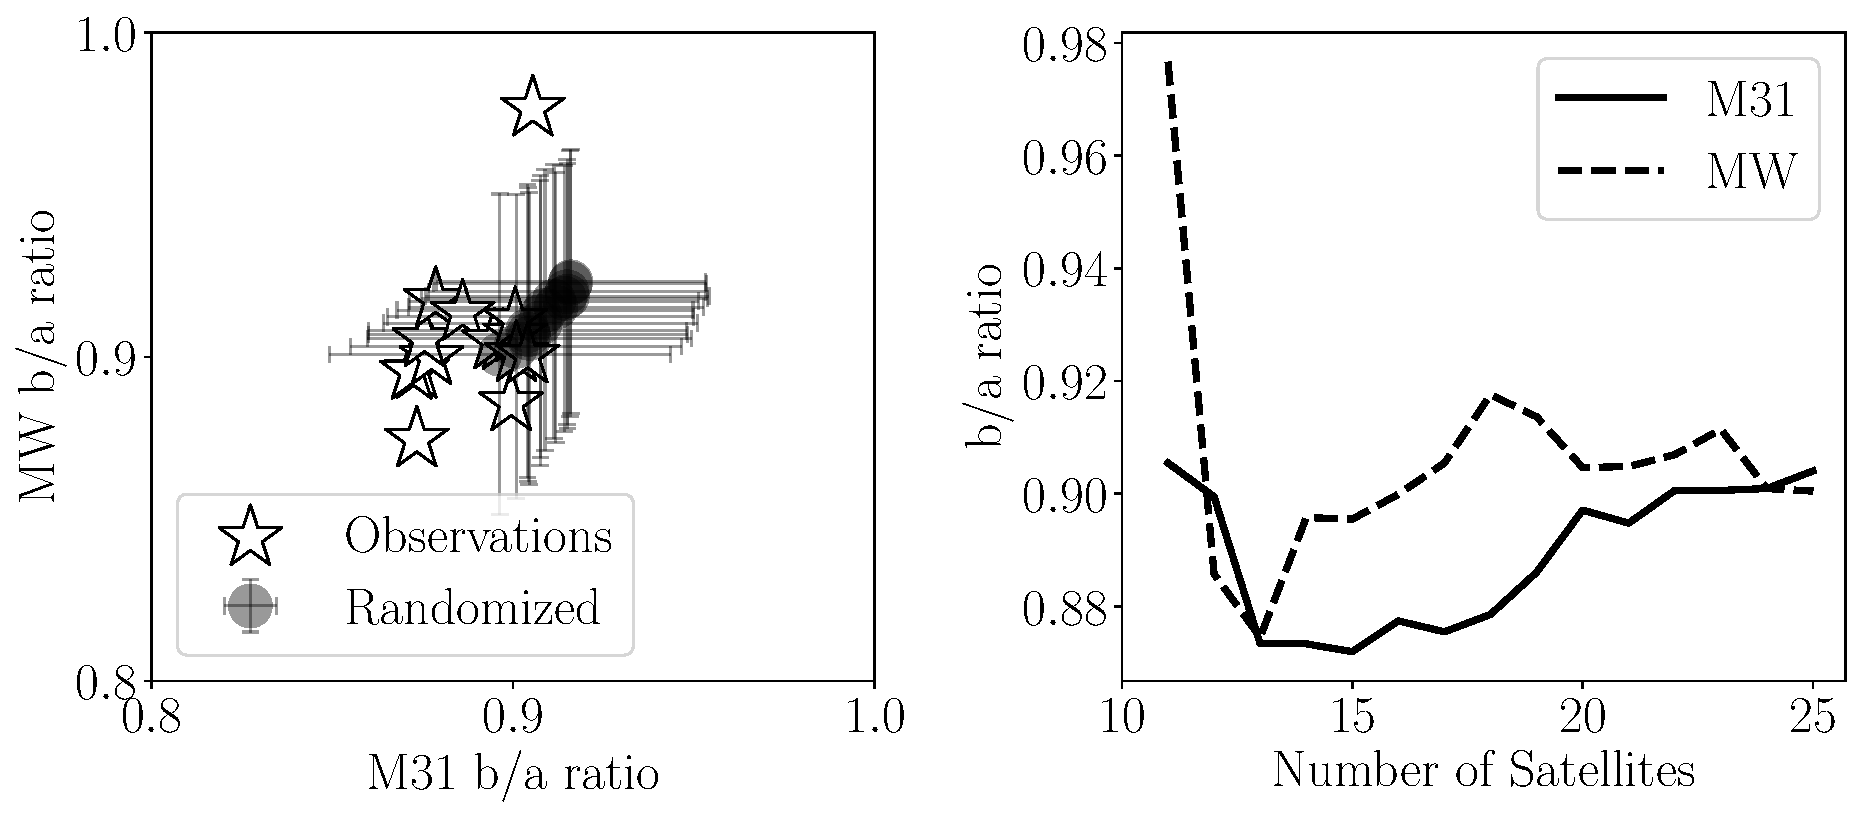
\includegraphics[width=0.7\textwidth]{ba_ratio_lg.pdf}
\caption{Basic characteristics for the MW and M31 satellite systems
\label{fig:general}}
\end{figure*}

\bibliographystyle{mnras}
\bibliography{Dwarfs}

%% Alignments between galaxies, satellite systems and haloes
%% https://arxiv.org/pdf/1605.01728.pdf

%M31 mass
%% https://arxiv.org/abs/1410.0017

%MW mass
%https://arxiv.org/abs/1407.1078


\end{document}

